% ACL long paper (review mode). Official style: github.com/acl-org/acl-style-files (acl.sty, acl_natbib.bst
% in this folder; acl_template_example.tex is the unmodified official example).
% Every number comes from exps/*/results/ (see exps/README.md). Figures: python paper_acl/make_figures.py
% (all six PDFs in figures/).
% Camera-ready: replace [review] by [final] and fill the author block.
\documentclass[11pt]{article}
% Numbered citations [1] (acl.sty loads natbib without options; ACL's default is author-year).
\PassOptionsToPackage{numbers,square,sort&compress}{natbib}
\usepackage[review]{acl}
\usepackage{times}
\usepackage{latexsym}
\usepackage[T1]{fontenc}
\usepackage[utf8]{inputenc}
\usepackage{microtype}
\usepackage{inconsolata}
\usepackage{graphicx}
\usepackage{amsmath,amssymb,amsthm}
\usepackage{booktabs}
\usepackage{multirow}
\usepackage{xcolor}

\newcommand{\todo}[1]{\textcolor{red}{[TODO: #1]}}
\newcommand{\Tr}{\mathrm{Tr}}
\newtheorem{proposition}{Proposition}

\title{Does Quantum Help Class-Incremental Learning?\\A Measurement-First Study}

\author{Anonymous ACL submission}

\begin{document}
\maketitle
\begin{abstract}
Quantum machine-learning components are often reported to improve classical
pipelines by less than the pipelines' own run-to-run variation. We study
whether quantum components help exemplar-free class-incremental learning with
a pre-trained model, under a protocol that resolves a few tenths of a point:
paired runs, all inference heads evaluated on one network, decision rules
fixed in advance, and a classical twin with the same inputs for every quantum
component. We test seven
placements: a projected quantum kernel as a steering metric, a separation
regulariser and a feature map; the Holevo quantity and a measurement-based
loss as training objectives; and a pretty-good measurement over class density
matrices, alone and fused with the classifier. Only one twin comparison has an
interval above zero, at $+0.04$ points. A read-only probe shows that the separation
kernel loses class information in its 8-qubit projection; repairing this lowers
accuracy. We prove that circuits after the encoding and state shrinkage
cannot change the measurement, and show across 61 stored runs that every
training-time change trades new-task for old-task accuracy. A calibrated fusion
of the classifier with a ridge score on the stored class statistics raises final
accuracy on four benchmarks by $0.38$ to $0.67$ points; the quantum score does
the same.
\end{abstract}

\section{Introduction}
\label{sec:intro}

Quantum machine learning (QML) offers models with no obvious classical
analogue, such as kernels defined by quantum feature
maps~\citep{huang2021power} and classifiers defined by measurements on quantum
states~\citep{hausladen1994pgm}. They are commonly evaluated by inserting one
into a strong classical pipeline and reporting the change in accuracy. In
continual learning these changes are often a few tenths of a point, about the
size of the pipeline's own run-to-run variation, and the classical alternative
to the quantum component is rarely tested~\citep{bowles2024better}. A recent
quantum method for class-incremental learning, for instance, reports single
numbers without variance~\citep{li2026qkd}.

We ask whether quantum components help \emph{exemplar-free class-incremental
learning} (CIL): a model learns new classes task after task, may not store
images of past tasks, and must classify all classes seen so far. The setting
suits quantum models for two reasons. The model must keep compact summaries of
past classes, and a density matrix is such a summary. Its main difficulty,
confusion between classes learned at different times, is a state-discrimination
problem. We start from RSIAT~\citep{rsiat}, a strong pre-trained baseline that
already stores one mean and one covariance per class.

Before testing any component we measured how much the baseline varies, and
built a protocol that resolves changes of $0.2$ points
(Section~\ref{sec:setup}). It pairs seeds and replicates, evaluates every
inference head on the same network, fixes decision rules before each run, and
gives every quantum component a \emph{classical twin} that receives the same
inputs. The first of these checks already overturned an earlier result of ours:
a $+0.36$ gain of a quantum-kernel variant over a single baseline run shrank to
$+0.06$ ($[-0.07,+0.18]$) under the protocol.

We then test quantum components wherever they can enter the pipeline
(Figure~\ref{fig:pipeline}). During training, a projected quantum kernel (PQK)
steers the base task or separates new features from old classes, and two
density-matrix objectives, the Holevo quantity and a measurement-based loss,
shape the adapter. At inference, the PQK serves as a feature map, and a
pretty-good measurement (PGM) over class density matrices classifies alone or
fused with the baseline classifier. Our contributions are:
\begin{itemize}
  \item \textbf{A measurement protocol} for small effects in CIL, and its
    application to seven quantum placements, each against its classical twin
    (Table~\ref{tab:quantum}). Only one twin comparison has an interval
    above zero, the PQK against the same circuit without entanglement, at $+0.04$ points of
    average accuracy; the PQK feature map loses up to $17$ points.
  \item \textbf{A diagnosis-then-repair study} of the quantum separation
    regulariser. A read-only probe locates its weaknesses (an 8-qubit
    projection that discards class information, saturated angles, a frozen
    kernel); repairing them makes average accuracy worse ($-0.07$, $[-0.11,-0.03]$).
  \item \textbf{Theory} explaining the measurement results: circuits applied
    after the encoding and the usual state shrinkage cannot change the PGM, so
    only the encoding remains as a quantum degree of freedom.
  \item \textbf{An analysis across 61 stored runs} showing that every
    training-time intervention we tried, quantum or not, trades accuracy on
    new tasks for accuracy on old tasks, and that only an inference-time fusion
    raises both. That fusion, with a classical or a quantum score, raises final
    accuracy on four benchmarks by $+0.38$ to $+0.67$ points.
\end{itemize}

\begin{figure*}[t]
\centering
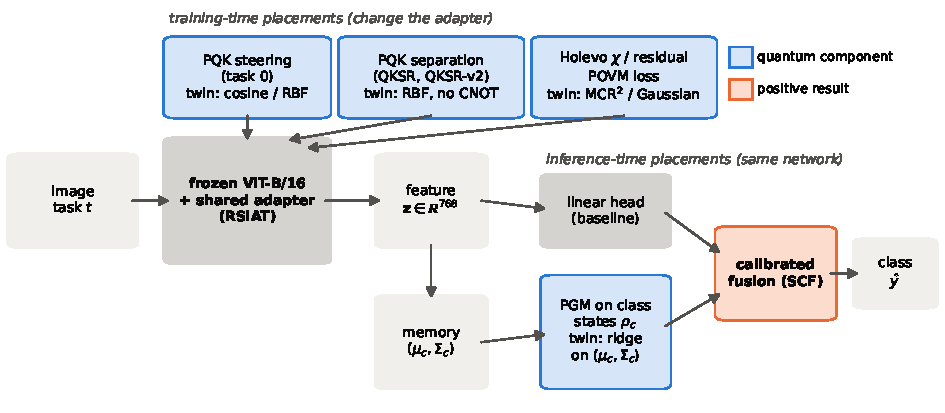
\includegraphics[width=0.92\textwidth]{figures/pipeline.pdf}
\caption{Where quantum components enter the RSIAT pipeline. Blue: quantum
placements, each listed with its classical twin. Training-time placements
change the shared adapter; inference-time placements are evaluated on the
same trained network. Orange: the calibrated score fusion (SCF), the only
component that raised both old- and new-task accuracy.}
\label{fig:pipeline}
\end{figure*}

\section{Related Work}
\label{sec:related}

\paragraph{Class-incremental learning with pre-trained models.}
With a frozen ViT, strong CIL methods tune a light adapter or prompt and keep
a classifier calibrated across tasks. Prompt-based methods select or compose
prompts per input~\citep{l2p,dualprompt,codaprompt}; adapter-based methods
expand task-specific subspaces~\citep{ease}, merge adapters~\citep{mos} or
compensate semantic shift~\citep{ssiat}. SLCA re-trains the classifier on Gaussian
samples of stored class statistics~\citep{zhang2023slca}; RanPAC uses random
projections and a closed-form ridge head~\citep{mcdonnell2023ranpac}; APER
combines frozen and adapted embeddings~\citep{zhou2024aper}. RSIAT, our
baseline, adds a representation-steering loss and drift compensation of the
stored means~\citep{rsiat}. \citet{smith2023closer} showed that, with a
pre-trained model, simple regularisers can match more elaborate ones, which
motivates simple classical baselines for every added component.

\paragraph{Exemplar-free drift and separation.}
Without exemplars, old classes survive only as statistics. ADC, LDC and EFC
compensate or constrain the drift of these
statistics~\citep{goswami2024adc,gomezvilla2024ldc,magistri2024efc}; AdaGauss
adapts the covariances and counters task-recency
bias~\citep{rypesc2024adagauss}. Closest to our separation regulariser,
PRL penalises the similarity between new features and old prototypes over all
pairs~\citep{shi2024prl}, and NAPA-VQ pushes apart neighbouring, confusable
classes~\citep{malepathirana2023napavq}. Rate-reduction objectives, the
classical counterpart of our Holevo objective, have also been applied to
incremental learning~\citep{wu2021rate}.

\paragraph{Quantum continual learning and benchmarking.}
Quantum continual learning has mostly studied small variational classifiers on
quantum or toy data, regularised as in classical
CIL~\citep{jiang2022qcl}. QKD routes distillation between task adapters with a
quantum gate on a pre-trained ViT~\citep{li2026qkd}. Projected kernels were
introduced to avoid the exponential concentration of global
fidelities~\citep{huang2021power,thanasilp2024concentration}; their bandwidth
controls their inductive bias~\citep{shaydulin2022bandwidth,canatar2022bandwidth},
and they can be trained by kernel--target alignment~\citep{hubregtsen2022qek}.
\citet{bowles2024better} found that out-of-the-box classical baselines
generally outperform the QML models they benchmarked. We follow their
recommendation of classical twins and add the paired, pre-registered
evaluation that small effects in CIL require.

\section{Task and Data}
\label{sec:task}

\paragraph{Task.}
Tasks $t=0,\dots,B-1$ bring disjoint label sets $\mathcal Y_t$. While learning
task $t$, only its training data is available. Afterwards the model classifies
test images of every class in $\mathcal C_t=\mathcal Y_0\cup\dots\cup\mathcal Y_t$,
with $C_t=|\mathcal C_t|$; $\tau(c)$ is the task that introduced class $c$.

\paragraph{Metrics.}
Let $A_k$ be the accuracy on $\mathcal C_k$ after task $k$, and $a_{k,j}$ the
accuracy on the classes of task $j$. We report the average incremental
accuracy $\bar A$, the final accuracy $A_B$ and the forgetting $F$:
\begin{align}
  \bar A&=\frac1B\sum_{k=0}^{B-1}A_k,\qquad A_B=A_{B-1},\label{eq:acc}\\
  F&=\frac1{B-1}\sum_{j<B-1}\Big(\max_{j\le k<B-1}a_{k,j}-a_{B-1,j}\Big).\label{eq:forget}
\end{align}
To read trade-offs, we also split the final per-task accuracy into an \emph{old} half
(the first $B/2$ tasks) and a \emph{new} half.

\paragraph{Data.}
We use four benchmarks: CIFAR-100~\citep{krizhevsky2009cifar} (10 tasks of 10
classes, 500 training images per class), ImageNet-R~\citep{hendrycks2021many}
(10 tasks of 20 classes, about 120 per class), ImageNet-A~\citep{hendrycks2021nae}
(10 tasks of 20 classes, about 30 per class) and CUB-200~\citep{wah2011cub}
(20 tasks of 10 classes, about 30 per class). We use partitions we can
redistribute: the standard CIFAR-100 split; a public fixed ImageNet-R split
(23\,918 training and 6\,082 test images); an 80/20 per-class split of
ImageNet-A with seed 67; and the official CUB-200 split (5\,994 / 5\,794).
Absolute numbers therefore differ slightly from the published ones
(Table~\ref{tab:main}). Every dataset is run with the seeds 1993, 2015 and 2026,
which also fix the class order. All free choices were made on a \emph{tuning
group} (ImageNet-R, seed 1993, three replicates) and then frozen; every other
dataset and seed is held out.

\section{Method}
\label{sec:method}

All circuits have at most 11 qubits and are simulated exactly as state
vectors. We therefore do not ask whether there is a quantum advantage, but
whether a quantum inductive bias helps CIL compared with its classical twin.

\subsection{Baseline}
\label{sec:baseline}
RSIAT~\citep{rsiat} adapts a frozen ViT-B/16~\citep{dosovitskiy2021vit} with
one adapter shared by all tasks and produces features $\mathbf z\in\mathbb R^{d}$,
$d=768$. Three parts matter here: a \emph{memory}
$\mathcal M_t=\{(\boldsymbol\mu_c,\Sigma_c)\}_{c\in\mathcal C_t}$, the only
information kept about past classes; a drift correction of the old means
after each task; and a cosine classifier re-trained after each task on
Gaussian samples from $\mathcal M_t$~\citep{zhang2023slca}, with logits
$\ell_c(\mathbf z)=s\cos(\mathbf w_c,\mathbf z)$. Its prediction
$\arg\max_c\ell_c$ is the \emph{linear head}. In incremental tasks the adapter
is trained with a CosFace loss on the new classes and an alignment loss
$\beta\,\|\mathbf z-\mathrm{AE}(\mathbf z^{\mathrm{old}})\|^2$ to the previous
network through an autoencoder.

\subsection{A Projected Quantum Kernel}
\label{sec:pqk}
A feature is mapped to $q=8$ angles
$\boldsymbol\theta(\mathbf z)=\pi\tanh(W\,\mathrm{LN}(\mathbf z)+\mathbf b)$,
loaded with $R_y$ rotations and followed by $L=2$ layers of trainable $R_y$
rotations and a ring of CNOTs. Following~\citet{huang2021power}, two states are
compared through their one-qubit reduced density matrices $\rho_j$:
\begin{equation}
  k(\mathbf z,\mathbf z')=\exp\Big(-\gamma\sum_{j=1}^{q}\big\|\rho_j(\mathbf z)-\rho_j(\mathbf z')\big\|_F^2\Big),
  \label{eq:pqk}
\end{equation}
with $\gamma$ calibrated from the median distance. The kernel enters at three
places (Figure~\ref{fig:pipeline}): (1)~as the similarity of the base task's
steering loss, trained with the adapter and then frozen; (2)~as a
\emph{separation regulariser} (QKSR) in incremental tasks, penalising the mean
kernel between stored old-class means (mapped through the autoencoder) and
current features; (3)~as a feature map for ridge heads fitted on the
classifier-alignment pseudo-features.

\paragraph{QKSR-v2.}
To test whether the regulariser fails for fixable reasons, a repaired variant
refits the kernel at the start of each task from stored statistics only: the
projection rows become the top Fisher-LDA directions of all class means and
covariances, scaled so that angles have a standard deviation of $0.8$ rad, and
$\gamma$ is set so that the median kernel between old means and new features
is $0.2$ (Appendix~\ref{app:hyper}).

\subsection{Training with Density-Matrix Objectives}
\label{sec:holevo}
Two further placements change the representation directly. Class states
$\rho_c$ are built from the memory (Eq.~\ref{eq:state} below) for old classes
and from a feature queue for new classes. The \emph{Holevo objective} adds
$-\lambda\chi$ to the adapter loss, with
\begin{equation}
  \chi=S(\bar\rho)-\frac1{C_t}\sum_{c\in\mathcal C_t}S(\rho_c),\qquad
  \bar\rho=\frac1{C_t}\sum_{c\in\mathcal C_t}\rho_c,
  \label{eq:holevo}
\end{equation}
and $S(\rho)=-\Tr\rho\log\rho$ the von Neumann entropy; its classical twin replaces $S$ by the coding rate of MCR$^2$~\citep{wu2021rate}.
The \emph{residual-POVM loss} measures new features with a POVM whose new-class
elements are restricted to the subspace left free by the old-class states;
its twin is a Gaussian log-likelihood classifier. $\lambda$ is calibrated once
so that the auxiliary gradient is half the classification gradient.

\subsection{CIL as State Discrimination}
\label{sec:qsd}
Let $\mathbf m_0$ and $s_0^2$ be the mean and covariance trace of task-0
features. A feature is lifted and normalised,
\begin{equation}
  \mathbf v(\mathbf z)=\begin{bmatrix}(\mathbf z-\mathbf m_0)/s_0\\1\end{bmatrix}\in\mathbb R^{D},\qquad
  \psi=\frac{\mathbf v}{\|\mathbf v\|},
  \label{eq:lift}
\end{equation}
with $D=769$, so that $\psi$ is the amplitude vector of a 10-qubit pure state.
A class becomes the second-moment state
\begin{equation}
  \begin{aligned}
  \rho_c&=\frac{\mathbb E_c[\mathbf v\mathbf v^{\top}]}{\mathbb E_c\|\mathbf v\|^2},\\
  \mathbb E_c[\mathbf v\mathbf v^{\top}]&=
  \begin{bmatrix}\tilde\Sigma_c+\tilde{\boldsymbol\mu}_c\tilde{\boldsymbol\mu}_c^{\top} & \tilde{\boldsymbol\mu}_c\\
  \tilde{\boldsymbol\mu}_c^{\top}&1\end{bmatrix},
  \end{aligned}
  \label{eq:state}
\end{equation}
computed from $\mathcal M_t$ alone ($\tilde{\boldsymbol\mu}_c$, $\tilde\Sigma_c$:
standardised moments). It needs no stored features and follows the drift
correction. The PGM~\citep{hausladen1994pgm} uses
\begin{equation}
  \begin{aligned}
  E_c&=\frac1{C_t}\,\bar\rho_\delta^{-1/2}\rho_c\,\bar\rho_\delta^{-1/2},\qquad
  \bar\rho_\delta=\bar\rho+\delta I,\\
  p(c\mid\mathbf z)&=\frac{\psi^{\top}E_c\psi}{\sum_{c'}\psi^{\top}E_{c'}\psi},
  \end{aligned}
  \label{eq:pgm}
\end{equation}
the Born probability of outcome $c$. A hierarchical variant first measures
the task with $E_T=\sum_{c\in\mathcal Y_T}E_c$, then the class inside it.

\paragraph{What the measurement can and cannot do.}
\begin{proposition}\label{prop:unitary}
For any unitary $U$ applied after the encoding, $p(c\mid\mathbf z)$ is unchanged.
\end{proposition}
\begin{proposition}\label{prop:shrink}
Replacing every $\rho_c$ by $(1-\varepsilon)\rho_c+\varepsilon\bar\rho$,
$\varepsilon\in[0,1)$, leaves $\arg\max_cp(c\mid\mathbf z)$ unchanged.
\end{proposition}
\noindent Proofs are in Appendix~\ref{app:proofs}. A variational circuit after
the amplitude encoding is a unitary, so training one cannot change the
classifier, and the usual state shrinkage does nothing. The PGM also coincides
with the least-squares measurement~\citep{eldar2001srm}. Only the encoding
remains as a quantum degree of freedom.

\subsection{Score Fusion and its Classical Twin}
\label{sec:fusion}
The classical twin of the PGM regresses one-hot targets on the class Gaussians
$\mathcal N(\boldsymbol\mu_c,\Sigma_c)$ with a ridge penalty, in the spirit
of~\citet{mcdonnell2023ranpac}. It has the closed form
\begin{equation}
  \begin{aligned}
  \Big(\sum_{c}(\Sigma_c+\boldsymbol\mu_c\boldsymbol\mu_c^{\top})+\lambda I\Big)W
  &=[\boldsymbol\mu_1,\dots,\boldsymbol\mu_{C_t}],\\
  g^{\mathrm R}_c(\mathbf z)&=\mathbf z^{\top}W_{:,c}.
  \end{aligned}
  \label{eq:ridge}
\end{equation}
A generative score $g$ (the PGM log-probability or $g^{\mathrm R}$) is fused
with the linear head:
\begin{equation}
  \begin{aligned}
  \hat y&=\arg\max_c\;\ell_c(\mathbf z)+w\,\kappa\,g_c(\mathbf z),\\
  \kappa&=\overline{\mathrm{sd}_c\,\ell_c}\,\big/\,\overline{\mathrm{sd}_c\,g_c},
  \end{aligned}
  \label{eq:fusion}
\end{equation}
where $\mathrm{sd}_c$ is the spread across classes, averaged over the current
task's training images; $\kappa$ needs no labels and makes $w$ invariant to
affine rescaling of $g$. We call this \emph{statistics-calibrated fusion}
(SCF). Neither score stores anything beyond $\mathcal M_t$.

\section{Experimental Setup}
\label{sec:setup}

\paragraph{How large is the noise?}
We ran the baseline four times on ImageNet-R with one seed; the base task was
identical and only the SGD randomness of later tasks changed. The spread is
$\bar A=87.35\pm0.14$ and $A_B=82.59\pm0.23$; on ImageNet-A the spread of
$\bar A$ is $0.38$. A single run against a single run therefore cannot resolve
effects below roughly half a point. With the authors' code and partitions, our
runs reproduce all twelve numbers of the baseline's main table ($\bar A$ and
$A_B$ on six benchmarks) to within $0.01$.

\paragraph{Protocol.}
Four rules govern every comparison.
\textbf{(1) Pair everything:} effects are paired differences over seeds or
replicates, with 95\% $t$-intervals.
\textbf{(2) Same network for all heads:} a component that only changes
inference is evaluated, after each task, on the same test features as the
linear head. Each head draws randomness from a private generator and the
global random state is restored afterwards; we check that the linear head
reproduces the logged curve digit for digit. The standard deviation of a
paired head difference falls from $0.2$ to $0.03$--$0.05$ points.
Training-time components cannot use this rule and are compared with baseline
runs of the same seed and replicate.
\textbf{(3) Decide before looking:} each round had a written specification
fixing components, hyper-parameters, the decision rule and the minimum effect
before it ran; Table~\ref{tab:tests} (Appendix~\ref{app:tests}) lists every
test, including the failed ones.
\textbf{(4) A classical twin for every quantum component}
(Figure~\ref{fig:pipeline}): an RBF kernel on the same angles or the same
circuit without CNOTs for the PQK; MCR$^2$ for the Holevo quantity; a Gaussian
classifier for the POVM loss; ridge regression on the same statistics for the
PGM. Beating the baseline is not enough, since the baseline does not use the
information that the component and its twin share.

\paragraph{Read-only probe.}
To diagnose the separation regulariser we added a probe that measures,
without changing training, the cosine between the adapter gradients of the
classification, alignment and separation losses every 10 steps, and, after
each task on 20 training images per class, how well distances in each space
separate classes (AUC of different-class versus same-class pairs). With the
probe on, weights are bit-identical to a run without it.

\paragraph{Implementation.}
Training-time comparisons of QKSR use three replicates on ImageNet-R seed 1993
in one computing environment; the Holevo and residual-POVM objectives were
screened with one run each, against a pre-registered stopping rule. All runs
used an NVIDIA RTX PRO 6000 Blackwell GPU (up to three runs in parallel),
PyTorch 2.11 and timm 1.0.29.
Hyper-parameters are in Appendix~\ref{app:hyper}.

\section{Results}
\label{sec:results}

\begin{table*}[t]
\centering
\small
\setlength{\tabcolsep}{3.5pt}
\begin{tabular}{llll}
\toprule
Placement & Comparison (A $-$ B) & $\Delta\bar A$ [95\% CI] & $n$ \\
\midrule
1. PQK, steering metric & PQK $-$ cosine (baseline), R & $+0.06$ [$-0.07$, $+0.18$] & 3 \\
\midrule
\multirow{5}{*}{2. PQK, separation (QKSR)} & current $-$ previous-model features, R & $-0.02$ [$-0.06$, $+0.03$] & 3 \\
 & PQK $-$ RBF on the same angles, R & $+0.07$ [$-0.01$, $+0.15$] & 3 \\
 & PQK $-$ same circuit without CNOTs, R & $+0.04$ [$+0.04$, $+0.05$] & 3 \\
 & repaired (QKSR-v2) $-$ QKSR, R & $-0.07$ [$-0.11$, $-0.03$] & 3 \\
 & repaired PQK $-$ repaired RBF, R & $-0.04$ [$-0.08$, $+0.00$] & 3 \\
\midrule
\multirow{4}{*}{3. PQK, feature map} & PQK ridge $-$ linear head, A & $-17.33$ [$-19.07$, $-15.59$] & 3 \\
 & PQK without CNOTs $-$ linear head, A & $-10.40$ [$-11.10$, $-9.71$] & 3 \\
 & random Fourier features $-$ linear head, A & $-1.41$ [$-2.52$, $-0.31$] & 3 \\
 & random projection $-$ linear head, A & $-1.24$ [$-2.29$, $-0.19$] & 3 \\
\midrule
4. Holevo objective & von Neumann $\chi$ $-$ MCR$^2$ twin, R & $+0.06$ & 1 \\
5. Residual-POVM loss & POVM $-$ Gaussian twin, R & twin diverged (see text) & 1 \\
\midrule
\multirow{3}{*}{6. PGM, stand-alone} & PGM $-$ ridge, same statistics, R+A & $+0.09$ [$-0.23$, $+0.40$] & 11 \\
 & moment states $-$ per-sample states, R+A & $+0.07$ [$-0.02$, $+0.16$] & 11 \\
 & two-copy encoding $-$ amplitude encoding & $-3.6$ (R), $-6.5$ (A) & 5+5 \\
7. PGM, fused (SCF) & PGM source $-$ ridge source, 4 datasets & $-0.04$ [$-0.17$, $+0.08$] & 12 \\
\bottomrule
\end{tabular}
\caption{Every quantum placement against its classical twin. $\Delta\bar A$ in
points over paired runs; R: ImageNet-R, A: ImageNet-A. Rows 4--5 are one-run
screening results (no interval).}
\label{tab:quantum}
\end{table*}

\begin{table*}[t]
\centering
\small
\setlength{\tabcolsep}{2.2pt}
\resizebox{\textwidth}{!}{%
\begin{tabular}{lcccccccccc}
\toprule
& \multicolumn{2}{c}{CIFAR-100} & \multicolumn{2}{c}{ImageNet-R} & \multicolumn{2}{c}{ImageNet-A}
& \multicolumn{2}{c}{CUB-200} & \multicolumn{2}{c}{Average} \\
\cmidrule(lr){2-3}\cmidrule(lr){4-5}\cmidrule(lr){6-7}\cmidrule(lr){8-9}\cmidrule(lr){10-11}
Method & $\bar A$ & $A_B$ & $\bar A$ & $A_B$ & $\bar A$ & $A_B$ & $\bar A$ & $A_B$ & $\bar A$ & $A_B$ \\
\midrule
\multicolumn{11}{l}{\textit{Reported by \citet{rsiat} (exemplar-free, authors' partitions, one run)}} \\
L2P~\citep{l2p} & 89.23 & 84.29 & 75.46 & 69.77 & 49.39 & 41.71 & 67.05 & 56.25 & 70.28 & 63.01 \\
DualPrompt~\citep{dualprompt} & 87.36 & 82.30 & 73.10 & 67.18 & 53.71 & 41.67 & 77.47 & 66.54 & 72.91 & 64.42 \\
CODA-Prompt~\citep{codaprompt} & 91.30 & 86.85 & 77.97 & 72.27 & 53.54 & 42.73 & 84.00 & 73.37 & 76.70 & 68.80 \\
APER+Adapter~\citep{zhou2024aper} & 90.94 & 85.75 & 75.82 & 67.95 & 60.47 & 49.37 & 92.21 & 86.73 & 79.86 & 72.45 \\
EASE~\citep{ease} & 92.35 & 87.76 & 81.74 & 76.17 & 65.34 & 55.04 & 92.23 & 86.81 & 82.91 & 76.45 \\
SLCA~\citep{zhang2023slca} & 94.09 & 91.53 & 81.17 & 77.00 & 68.66 & 58.74 & 89.51 & 82.19 & 83.36 & 77.36 \\
RanPAC~\citep{mcdonnell2023ranpac} & 94.35 & 90.86 & 82.98 & 77.94 & 69.32 & 61.82 & 93.13 & 89.40 & 84.94 & 80.00 \\
MOS~\citep{mos} & 94.75 & 91.70 & 82.96 & 77.93 & 69.13 & 59.12 & 93.49 & 90.12 & 85.08 & 79.72 \\
SSIAT~\citep{ssiat} & 94.35 & 91.35 & 83.63 & 79.38 & 70.83 & 62.43 & 93.38 & 89.53 & 85.55 & 80.67 \\
RSIAT~\citep{rsiat} & 95.15 & 92.20 & 86.92 & 82.75 & 74.89 & 66.23 & 93.99 & 90.59 & 87.74 & 82.94 \\
\midrule
\multicolumn{11}{l}{\textit{Our runs (our partitions, mean $\pm$ SD over three seeds)}} \\
RSIAT (ours) & 95.02{\tiny$\pm$.21} & 92.03{\tiny$\pm$.19} & 87.11{\tiny$\pm$.49} & 82.55{\tiny$\pm$.05}
 & 74.26{\tiny$\pm$1.1} & 67.02{\tiny$\pm$1.1} & 93.53{\tiny$\pm$.79} & 88.47{\tiny$\pm$.31} & 87.48 & 82.52 \\
SCF, ridge (classical) & 95.22{\tiny$\pm$.20} & \textbf{92.41}{\tiny$\pm$.21} & 87.42{\tiny$\pm$.46} & 83.03{\tiny$\pm$.24}
 & \textbf{75.12}{\tiny$\pm$1.2} & \textbf{67.69}{\tiny$\pm$0.9} & \textbf{93.54}{\tiny$\pm$.88} & \textbf{88.85}{\tiny$\pm$.22} & \textbf{87.83} & \textbf{83.00} \\
SCF, PGM (quantum) & \textbf{95.23}{\tiny$\pm$.22} & 92.34{\tiny$\pm$.16} & \textbf{87.50}{\tiny$\pm$.43} & \textbf{83.07}{\tiny$\pm$.42}
 & 74.89{\tiny$\pm$1.0} & 67.65{\tiny$\pm$1.3} & 93.50{\tiny$\pm$.84} & 88.57{\tiny$\pm$.30} & 87.78 & 82.91 \\
\midrule
$\Delta$ ridge & $+$.20 {\tiny[.12,.28]} & $+$.38 {\tiny[.08,.69]} & $+$.32 {\tiny[.12,.51]} & $+$.48 {\tiny[.02,.94]}
 & $+$.85 {\tiny[.62,1.08]} & $+$.67 {\tiny[$-$.20,1.54]} & $+$.02 {\tiny[$-$.24,.27]} & $+$.38 {\tiny[.16,.61]} & $+$.35 & $+$.48 \\
$\Delta$ PGM & $+$.22 {\tiny[.15,.28]} & $+$.31 {\tiny[.18,.43]} & $+$.39 {\tiny[.25,.53]} & $+$.52 {\tiny[$-$.41,1.45]}
 & $+$.63 {\tiny[$-$.10,1.36]} & $+$.62 {\tiny[$-$.08,1.32]} & $-$.03 {\tiny[$-$.18,.12]} & $+$.10 {\tiny[.05,.16]} & $+$.30 & $+$.39 \\
\bottomrule
\end{tabular}}
\caption{Exemplar-free CIL with ViT-B/16-IN21K on four benchmarks. Top: results
reported in Table~1 of \citet{rsiat} on the authors' partitions (one run each);
they are not directly comparable with ours. Bottom: our runs, mean $\pm$ SD over
seeds 1993, 2015 and 2026; $\Delta$: paired difference of score fusion to RSIAT
in the same runs, with 95\% CI. Fusion weights were frozen on the tuning group
(ridge $w=0.25$, PGM $w=0.5$). Bold: best of our runs.}
\label{tab:main}
\end{table*}

\paragraph{No quantum component credibly beats its twin.}
Table~\ref{tab:quantum} is the main result of this study. Of the comparisons
with intervals, all but one contain zero or lie below it. The exception, the
separation kernel against the same circuit without CNOTs, is $+0.04$ points of
$\bar A$; the PQK also keeps old tasks better than the RBF twin (final accuracy
$+0.22$, $[+0.05,+0.39]$), but its gain in $\bar A$ is not resolved. The PQK as
a feature map and the richer two-copy encoding are clearly harmful. The PGM
matches ridge regression on the same statistics, alone and fused, as the
least-squares equivalence and Propositions~\ref{prop:unitary}--\ref{prop:shrink}
predict. The two training-time density-matrix objectives were stopped at
screening: the Holevo objective did not change final accuracy ($-0.18$ against
the four-run baseline mean, pre-registered threshold $+0.5$) and its classical
twin did as well. The Gaussian twin of the POVM loss diverged in task~1,
because its saturated softmax produced a near-zero gradient during the
calibration of $\lambda$, which then hit its upper bound; that comparison is
therefore not valid.

\paragraph{Repairing the separation kernel does not help.}
Against the baseline in the same environment, QKSR changes $\bar A$ by $+0.05$
($[-0.18,+0.28]$, $n=3$) while reducing forgetting by $0.54$
($[0.38,0.69]$). Its repaired version, which removes the weaknesses found by
the probe (Section~\ref{sec:qksr-analysis}), is worse than QKSR by $0.07$
points, and with the repair the PQK and its RBF twin become indistinguishable.

\paragraph{A classical fusion helps.}
Table~\ref{tab:main} gives the fusion results, which do not depend on the
quantum source. Final accuracy rises on all four datasets, by $+0.38$ to
$+0.67$ with the ridge source, and the interval excludes zero on three.
Average accuracy rises on CIFAR-100, ImageNet-R and ImageNet-A but not on
CUB-200, where the gain appears only in the last 3 of 20 stages; the
pre-registered transfer test to the two held-out datasets therefore failed
(Appendix~\ref{app:tests}). The ridge and PGM sources track each other at every
stage (Figure~\ref{fig:stage}, Appendix~\ref{app:figures}).

\paragraph{Position among published methods.}
Table~\ref{tab:main} and Figure~\ref{fig:comparison} place our runs next to
nine exemplar-free methods with the same backbone and task splits, as reported
by \citet{rsiat}. These numbers come from other partitions and single runs, so
they locate our results but do not test them; on the authors' partitions our
code reproduces the published RSIAT row to within $0.01$. With this caveat,
fusion's final accuracy is above every reported method on CIFAR-100,
ImageNet-R and ImageNet-A, and below the four strongest on CUB-200, where our
baseline is itself $2.1$ points below the published one. Exemplar-based methods
are compared in Appendix~\ref{app:exemplar}.

\begin{figure*}[t]
\centering
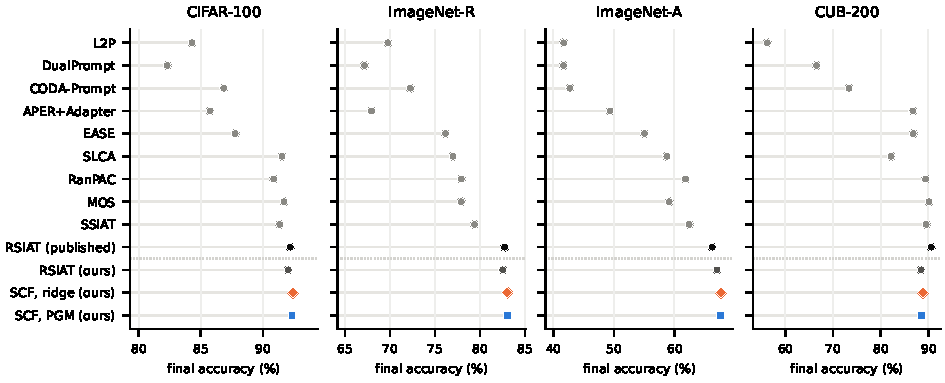
\includegraphics[width=\textwidth]{figures/comparison.pdf}
\caption{Final accuracy of nine exemplar-free methods (grey) and RSIAT (black) as reported by \citet{rsiat}, and of our runs (below the dotted line; mean over three seeds, our partitions). Orange: fusion with the classical ridge score; blue: with the quantum PGM score. Published and our numbers use different partitions.}
\label{fig:comparison}
\end{figure*}

\section{Analysis}
\label{sec:analysis}

\subsection{Where the Baseline Loses Accuracy}
\label{sec:gap}
On ImageNet-R, training once on all 200 classes gives $A_B=86.52$, $3.9$ points
above the baseline (per-task values in Table~\ref{tab:gap},
Appendix~\ref{app:gap}). The gap sits in the oldest classes: tasks~0 and~1
lose $9.0$ and $8.3$ points, while the newest task matches joint training. The
extra errors are cross-task: per pair of classes, the ratio of cross-task to
within-task confusions is $1.38$ for the baseline and $0.90$ for joint
training. Exact statistics do not close the gap: giving the classifier
alignment the oracle statistics of old classes adds only $+0.195$ to $\bar A$;
it lifts task~0 from $80.1$ to $87.1$, but newer tasks drop. The remaining
errors are overlaps between tasks in the learned representation.

\subsection{Every Training-Time Change Trades New for Old}
\label{sec:frontier}

\begin{figure}[t]
\centering
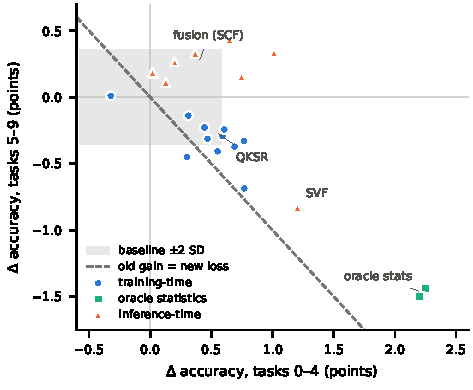
\includegraphics[width=\columnwidth]{figures/frontier.pdf}
\caption{Change of final accuracy on the old (tasks 0--4) and new (tasks 5--9)
halves against the baseline, ImageNet-R seed 1993, for every stored run and
head. Grey box: $\pm2$ SD of the five stored baseline runs of this seed. Points on the dashed line
gain on old tasks exactly what they lose on new ones.}
\label{fig:frontier}
\end{figure}

Figure~\ref{fig:frontier} places every stored run and head on ImageNet-R seed
1993 by the change of its old- and new-half accuracy (61 stored runs over all
datasets enter the analysis). This analysis is post hoc; its reading criteria
were written before running the script.
\begin{itemize}
  \item \emph{Training-time interventions trade.} None of the 11 runs that
    change the adapter (6 QKSR, 3 Holevo, 2 POVM) raises both halves. All 5
    that move the old half by more than two standard deviations keep final
    accuracy within two standard deviations; they lose a median $0.49$ points
    on new tasks per point gained on old ones, so $\bar A$ stays flat.
  \item \emph{Oracle statistics move furthest along the same line}: old
    $+2.2$, new $-1.5$.
  \item \emph{Only fusion raises both halves}: 28 of 37 inference-time points
    over all datasets. A snapshot-view head, which fuses the linear
    head with ridge scores on the features of the frozen task-0 network, is
    also inference-time but trades like the training-time changes, so our pre-registered criterion, which
    grouped the two, was not met.
\end{itemize}
The quantum regularisers therefore did not fail for quantum reasons: within
a shared adapter, separating old from new classes moves accuracy along a
trade-off curve rather than above it.

\subsection{Why the Separation Kernel Fails}
\label{sec:qksr-analysis}

\begin{table}[t]
\centering
\small
\setlength{\tabcolsep}{3pt}
\begin{tabular}{lr}
\toprule
Probe quantity (median over tasks 1--9) & Value \\
\midrule
Class AUC, cosine on $\mathbf z$ (768-d) & 0.95 \\
Class AUC, Euclidean on $\mathbf z$ & 0.85 \\
Class AUC, RBF on the 8 angles & 0.72 \\
Class AUC, PQK distance & 0.59 \\
\quad PQK at task 0 / task 9 & 0.76 / 0.57 \\
Angles with $|\theta|>0.9\pi$ & 43\% \\
Between-class scatter in projector span & $3.9\times$ random \\
Kernel, top-5 nearest old means / all & 0.85 / 0.56 \\
\midrule
cos(classification, separation gradient) & $-0.002$ \\
$\|$separation$\|$ / $\|$classification$\|$ gradient & 0.24 \\
cos(classification, alignment gradient) & $-0.14$ \\
\bottomrule
\end{tabular}
\caption{Read-only probe of the QKSR run (ImageNet-R, seed 1993). AUC: probability
that a different-class pair is farther apart than a same-class pair.}
\label{tab:probe}
\end{table}

Table~\ref{tab:probe} locates the weaknesses of the separation kernel. The
768-dimensional features separate classes well, but the 8-angle projection
keeps little of it, and the circuit loses more (AUC $0.85\to0.72\to0.59$).
Because the projection is frozen after task~0, it degrades from task to task
(Figure~\ref{fig:probe-auc}, Appendix~\ref{app:figures}),
and 43\% of the angles saturate the $\tanh$. The separation gradient is nearly
orthogonal to the classification gradient and a quarter of its size, so it
moves the adapter in directions irrelevant to classification; there is no
gradient conflict for methods such as auxiliary-gradient
projection~\citep{dery2021attittud} to remove, and tuned loss weights
generally match such methods anyway~\citep{xin2022mtl,kurin2022unitary}. The repair fixes the measured
weaknesses: the kernel used in training is no longer concentrated (mean
$0.06$--$0.11$ instead of $0.55$), yet accuracy drops. One reading, which we
have not tested, is that QKSR's small benefit on old tasks comes from a diffuse
push away from all old classes, which a sharper kernel concentrates on a few
near pairs. Unexpectedly, the alignment gradient opposes the classification
gradient at every probed step, in the baseline as well ($-0.15$); it is a
candidate source of the trade-off of Section~\ref{sec:frontier}.

\subsection{Error Analysis of the Measurement}
\label{sec:errors}
In the base task, where there is no drift, the PGM matches the linear head on
ImageNet-R ($-0.31$, $[-0.77,+0.15]$) and beats ridge on the same statistics
($+0.68$, $[+0.44,+0.92]$). As tasks accumulate, its deficit to the linear head
grows linearly to $-2.79$; the extra errors are old images assigned to newer
tasks ($11.5\%$ of the test set against $9.9\%$ for the linear head).
Transporting the states with a fitted channel does not change this, and oracle
states lift task~0 by $2.8$--$6.5$ points but $A_B$ by only $+0.64$. The
hierarchical measurement removes about two thirds of the deficit ($+0.33$,
$[+0.02,+0.64]$ over the flat PGM).

Stand-alone, every generative score is worse than the linear head, but they
err on different images. On ImageNet-R the PGM and the linear head disagree on
$14\%$ of the test images: the linear head is right on $5.8\%$ of them, the PGM
on $3.2\%$, and neither on $5.4\%$. Calibration is what lets fusion use this:
an uncalibrated sum follows the linear head on $87\%$ of the disagreements,
because Born probabilities are much flatter than a softmax at scale $s$, and
gains only $+0.25$ (ImageNet-R) and $+0.44$ (ImageNet-A).
\todo{Qualitative examples: test images on which the linear head and the
fused head disagree (images are not stored with the logs; recover them from
the fixed ImageNet-R split by test index).}

\section{Conclusion}
\label{sec:conclusion}

We asked whether quantum components help exemplar-free class-incremental
learning, and answered with a protocol that resolves a few tenths of a point.
Across seven placements, no quantum component credibly beats the classical
method that receives the same inputs; the one interval above zero is
$+0.04$ points. Three lessons generalise beyond this baseline. First, measure
the noise before claiming a gain: an earlier $+0.36$ of ours vanished, and
evaluating all inference heads on one network cuts the noise of a comparison
to $0.03$--$0.05$ points. Second, test the classical twin: the PGM fusion beat
the baseline but not ridge regression on the same statistics. Third, know which
degrees of freedom are real: circuits after an amplitude encoding and state
shrinkage cannot change the measurement, and repairing a regulariser's measured
weaknesses does not move it past a trade-off that the shared adapter imposes.
The state-discrimination view did produce a useful classical result: the class
statistics kept by exemplar-free methods carry information the aligned
classifier does not use, and a calibrated fusion recovers part of it without
training or new memory.

\section*{Limitations}

\begin{itemize}
  \item \textbf{One baseline.} All components were inserted into RSIAT with a
    single shared adapter. The trade-off of Section~\ref{sec:frontier} may not
    hold for methods with one adapter per task, such as QKD~\citep{li2026qkd},
    which we could not run because its released repository contains no code.
  \item \textbf{Narrow evidence for the training-time components.} QKSR and
    its repair were compared on ImageNet-R with one seed and three
    replicates; the Holevo and residual-POVM objectives were screened with one
    run each and stopped; the Gaussian twin of the POVM loss diverged because
    of our calibration of $\lambda$, so that comparison is missing. The repair
    was tested at one setting (8 qubits, angle spread $0.8$ rad, target kernel
    $0.2$), without a sweep.
  \item \textbf{Changing environment.} The computing environment changed
    between rounds: QKSR's base task reached $96.33\%$ in one environment and
    $96.05\%$ in the next. We therefore compare training-time components only
    with runs from the same environment, which halves the usable runs for
    some comparisons.
  \item \textbf{Post-hoc trade-off analysis.} Figure~\ref{fig:frontier} was
    drawn from runs we had already seen, mostly on one dataset and seed; it is
    exploratory, and the pre-registered criterion separating inference-time
    from training-time changes was not met.
  \item \textbf{Small simulated circuits.} Our circuits have at most 11 qubits
    and are simulated exactly. The negative results concern these placements
    and encodings, not quantum models in general or hardware effects.
  \item \textbf{Fusion transfer.} The fusion's gain in average accuracy did
    not transfer to CUB-200, and its pre-registered transfer test to the
    held-out datasets failed.
  \item \textbf{No qualitative inspection.} Images are not stored with our
    logs, so we report error statistics but no inspected examples.
\end{itemize}

\section*{Ethics Statement}

This work uses four public image benchmarks (CIFAR-100, ImageNet-R,
ImageNet-A, CUB-200) under their research licenses, and a publicly released
pre-trained ViT-B/16. It involves no human subjects and no personal data.
The study's main risk is the opposite of harm from deployment: overstated
claims about quantum methods, which we address by reporting every
pre-registered test, including the failed ones. All experiments ran on one GPU
model; \todo{report total GPU hours from the run logs}.
\todo{Declare the use of AI assistants in coding and writing, following the
venue's policy.}


\bibliography{references}

\appendix
\section{Proofs}
\label{app:proofs}

\begin{proposition}[valid states]
$\rho_c$ in Eq.~\eqref{eq:state} is positive semi-definite with unit trace. It
is the mixture $\mathbb E_c[\pi(\mathbf z)\psi\psi^{\top}]$ of the encoded pure
states with weights $\pi(\mathbf z)=\|\mathbf v(\mathbf z)\|^2/\mathbb E_c\|\mathbf v\|^2$.
\end{proposition}
\begin{proof}
$\mathbf v\mathbf v^{\top}=\|\mathbf v\|^2\psi\psi^{\top}$. Taking expectations
gives a non-negative combination of rank-one projectors with trace
$\mathbb E_c\|\mathbf v\|^2$.
\end{proof}

\begin{proof}[Proof of Proposition~\ref{prop:unitary}]
$\bar\rho_\delta\mapsto U\bar\rho_\delta U^{\dagger}$. Matrix functions commute
with unitary conjugation, so $E_c\mapsto UE_cU^{\dagger}$ and
$(U\psi)^{\dagger}UE_cU^{\dagger}U\psi=\psi^{\dagger}E_c\psi$.
\end{proof}

\begin{proof}[Proof of Proposition~\ref{prop:shrink}]
$\bar\rho$ and $\bar\rho_\delta$ do not change. Each numerator becomes
$(1-\varepsilon)\psi^{\top}E_c\psi+\varepsilon\psi^{\top}\bar E\psi$ with
$\bar E=\frac1{C_t}\bar\rho_\delta^{-1/2}\bar\rho\,\bar\rho_\delta^{-1/2}$; the
denominator is unchanged. This is one increasing affine map applied to every
class alike.
\end{proof}

\begin{proposition}[scale invariance of the fusion]
For any $a>0$ and class-independent $b(\mathbf z)$, replacing $g_c$ by $a\,g_c+b$
leaves $\hat y$ in Eq.~\eqref{eq:fusion} unchanged.
\end{proposition}
\begin{proof}
$\kappa\mapsto\kappa/a$, so $\kappa g_c\mapsto\kappa g_c+\kappa b/a$, and the added
term does not depend on $c$.
\end{proof}
\noindent Hence the same weight $w$ means the same thing for both sources and on
every dataset, which makes a frozen weight a fair comparison of the PGM and its
twin. For the PGM, the fused softmax is $p_{\mathrm{lin}}(c\mid\mathbf z)\,p(c\mid\mathbf z)^{w\kappa}$
up to normalisation; for integer $k$, $p^k$ is the Born probability of
$E_c^{\otimes k}$ on $k$ copies, so $w\kappa$ acts as an effective number of
measured copies.

\section{Hyper-parameters}
\label{app:hyper}

\begin{table}[h]
\centering
\small
\setlength{\tabcolsep}{2.5pt}
\begin{tabular}{lcccc}
\toprule
 & CIFAR & IN-R & IN-A & CUB \\
\midrule
Epochs, task 0 / later & 10 / 30 & 30 / 30 & 20 / 15 & 20 / 30 \\
Batch size & 64 & 48 & 48 & 128 \\
Learning rate (SGD) & 0.0185 & 0.0067 & 0.0067 & 0.0377 \\
Warm-up epochs & 7 & 4 & 3 & 9 \\
Alignment weight $\beta$ & 1.0 & 3.0 & 3.0 & 1.5 \\
Separation weight & 0.4 & 1.5 & 6.0 & 0.75 \\
Steering weight & 0.2 & 0.5 & 1.0 & 0.2 \\
CosFace scale / margin & 40 / 0.1 & 50 / 0.2 & 30 / 0.3 & 20 / 0.1 \\
Autoencoder code size & 256 & 384 & 128 & 768 \\
Classifier-alignment epochs & 10 & 10 & 10 & 10 \\
\bottomrule
\end{tabular}
\caption{Baseline hyper-parameters (the RSIAT configurations, unchanged).}
\label{tab:hyper}
\end{table}

\paragraph{Components.}
Table~\ref{tab:hyper} lists the baseline settings. The PQK uses 8 qubits, 2
variational layers, one-qubit reduced states, and a bandwidth bounded within a
factor of 10 of the inverse median distance on 512 calibration images. The
PGM uses $\delta=0.1/2^{10}$; the ridge twin $\lambda=0.1\,\mathrm{tr}(\cdot)/d$; the
fusion weight grid is $\{0.25,0.5,1,2,4\}$, with $w=0.25$ (ridge) and $w=0.5$
(PGM) chosen on the tuning group. The Holevo and POVM objectives use a feature
queue of up to 256 images per new class and a weight $\lambda$ calibrated in
the first epoch of task~1 so that the auxiliary gradient norm is half the
classification gradient norm, with a linear warm-up. QKSR-v2 refits the
projection at the start of every task by Fisher LDA on all stored class means
and covariances (ridge $10^{-3}\,\mathrm{tr}(S_W)/d$), scales each projection
row to an angle spread of $0.8$ rad, removes the LayerNorm, and sets $\gamma$ so
that the median kernel between old means and new features is $0.2$.

\section{Per-Task Gap to Joint Training}
\label{app:gap}

\begin{table}[h]
\centering
\small
\setlength{\tabcolsep}{2pt}
\resizebox{\columnwidth}{!}{%
\begin{tabular}{lrrrrrrrrrr}
\toprule
Task & 0 & 1 & 2 & 3 & 4 & 5 & 6 & 7 & 8 & 9\\
\midrule
Joint  & 89.1 & 88.7 & 86.4 & 86.4 & 83.2 & 86.0 & 85.8 & 87.0 & 85.4 & 85.8\\
CIL    & 80.1 & 80.4 & 82.7 & 82.3 & 78.8 & 82.7 & 85.3 & 84.2 & 83.9 & 86.2\\
Oracle & 87.1 & 83.1 & 83.5 & 82.2 & 79.1 & 81.6 & 84.7 & 82.9 & 82.1 & 83.6\\
\midrule
J$-$C & $+9.0$ & $+8.3$ & $+3.7$ & $+4.1$ & $+4.4$ & $+3.3$ & $+0.5$ & $+2.9$ & $+1.6$ & $-0.3$\\
\bottomrule
\end{tabular}}
\caption{Final accuracy (\%) per task on ImageNet-R; task 0 holds the oldest
classes. CIL: baseline, 4 replicates. Oracle: classifier alignment with exact
old-class statistics, 2 runs. Joint: one task with all 200 classes.}
\label{tab:gap}
\end{table}

Table~\ref{tab:gap} gives the per-task values behind Section~\ref{sec:gap}.

\section{Pre-Registered Tests}
\label{app:tests}

\begin{table*}[t]
\centering
\small
\begin{tabular}{llll}
\toprule
Test & Runs & $\Delta$ [95\% CI] & Outcome \\
\midrule
SCF-PGM beats the baseline by $\ge0.3$ $\bar A$, held out & R, A; 8 & $+0.46$ [$+0.28$, $+0.64$] & passed \\
Transfer to unseen datasets, SCF-ridge & CIFAR, CUB; 6 & $+0.11$ [$-0.02$, $+0.24$] & \textbf{failed} \\
Transfer to unseen datasets, SCF-PGM & CIFAR, CUB; 6 & $+0.09$ [$-0.05$, $+0.24$] & \textbf{failed} \\
PGM better than ridge as fusion source & all; 12 & $-0.04$ [$-0.17$, $+0.08$] & \textbf{failed} \\
Oracle states worth $\ge1$ point of $A_B$ & R, A; 11 & $+0.64$ [$+0.48$, $+0.80$] & \textbf{failed} \\
Holevo objective: $A_B$ $\ge+0.5$ over baseline (screening) & R; 1 & $-0.18$ & \textbf{failed}, stopped \\
Holevo + POVM: $A_B$ $\ge+0.5$ over baseline (screening) & R; 1 & $+0.11$ & \textbf{failed}, stopped \\
QKSR: PQK beats RBF twin in $\bar A$ & R; 3 & $+0.07$ [$-0.01$, $+0.15$] & inconclusive \\
QKSR: PQK beats circuit without CNOTs in $\bar A$ & R; 3 & $+0.04$ [$+0.04$, $+0.05$] & passed \\
QKSR-v2: old and new halves up, $\bar A$ CI $>0$ vs QKSR & R; 3 & $-0.07$ [$-0.11$, $-0.03$] & \textbf{failed} \\
Training-time changes stay on the trade-off line (post hoc) & R; 11 & 5 of 5 & held \\
Inference-time changes cross it (post hoc) & R; 9 & $z$ gap $0.83<1$ & \textbf{not met} \\
\bottomrule
\end{tabular}
\caption{Every pre-registered test, in the order it was run.}
\label{tab:tests}
\end{table*}

Table~\ref{tab:tests} lists every pre-registered test with its outcome.

\section{Comparison with Exemplar-Based Methods}
\label{app:exemplar}

\begin{table}[h]
\centering
\small
\setlength{\tabcolsep}{3pt}
\begin{tabular}{lcccc}
\toprule
& \multicolumn{2}{c}{ImageNet-R} & \multicolumn{2}{c}{CIFAR-100} \\
\cmidrule(lr){2-3}\cmidrule(lr){4-5}
Method & $\bar A$ & $A_B$ & $\bar A$ & $A_B$ \\
\midrule
\multicolumn{5}{l}{\textit{Reported by \citet{rsiat}; 20 exemplars per class}} \\
iCaRL~\citep{icarl} & 72.42 & 60.67 & 82.46 & 73.87 \\
DER~\citep{der} & 80.48 & 74.32 & 86.04 & 77.93 \\
FOSTER~\citep{foster} & 81.34 & 74.48 & 89.87 & 84.91 \\
MEMO~\citep{memo} & 74.80 & 66.62 & 84.08 & 75.79 \\
TagFex~\citep{tagfex} & 83.23 & 78.45 & 92.17 & 89.26 \\
\midrule
\multicolumn{5}{l}{\textit{Exemplar-free}} \\
RSIAT, published~\citep{rsiat} & 86.92 & 82.75 & 95.15 & 92.20 \\
RSIAT (ours, 3 seeds) & 87.11 & 82.55 & 95.02 & 92.03 \\
SCF, ridge (ours) & 87.42 & 83.03 & 95.22 & 92.41 \\
SCF, PGM (ours) & 87.50 & 83.07 & 95.23 & 92.34 \\
\bottomrule
\end{tabular}
\caption{Exemplar-based methods with ViT-B/16-IN21K (Table~2 of \citet{rsiat},
authors' partitions, one run) next to exemplar-free results. Our rows use our
partitions and average three seeds.}
\label{tab:exemplar}
\end{table}

Table~\ref{tab:exemplar} shows that, with a pre-trained ViT, the exemplar-free
methods reach higher accuracy than the reported exemplar-based ones on both
benchmarks; the same caveat on partitions as in Table~\ref{tab:main} applies.

\section{Additional Figures}
\label{app:figures}

\begin{figure*}[t]
\centering
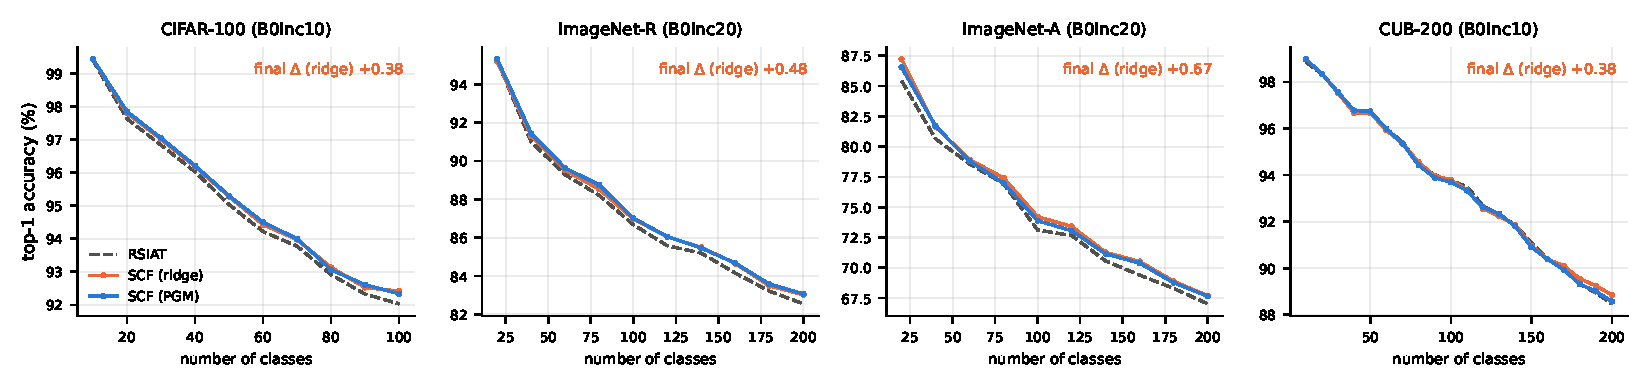
\includegraphics[width=\textwidth]{figures/accuracy_curves.pdf}
\caption{Accuracy after each task against the number of classes seen, mean over
three seeds: RSIAT (ours, dashed) and score fusion with the ridge (orange) and
PGM (blue) sources.}
\label{fig:curves}
\end{figure*}

\begin{figure*}[t]
\centering
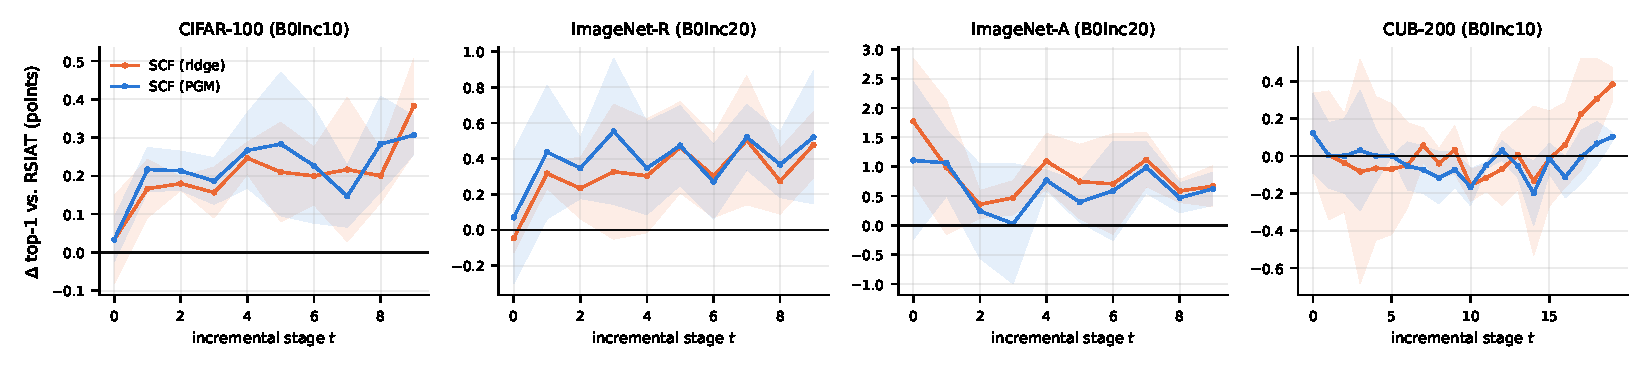
\includegraphics[width=\textwidth]{figures/delta_per_stage.pdf}
\caption{Paired gain of fusion over the baseline at each stage, mean $\pm$ SD
over three seeds. Orange: ridge source (classical). Blue: PGM source (quantum).}
\label{fig:stage}
\end{figure*}

\begin{figure}[t]
\centering
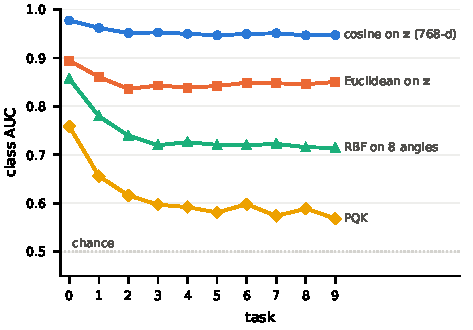
\includegraphics[width=\columnwidth]{figures/probe_auc.pdf}
\caption{Class separability measured by the probe after each task of the QKSR
run (ImageNet-R, seed 1993): probability that a different-class pair is farther
apart than a same-class pair, for distances on the 768-d feature, on the 8
projected angles, and in the PQK.}
\label{fig:probe-auc}
\end{figure}

Figure~\ref{fig:curves} gives the accuracy curves behind Table~\ref{tab:main},
and Figure~\ref{fig:stage} the paired gain of fusion per stage: it is positive
from the second stage on CIFAR-100 and ImageNet-R, largest at the first stage
on ImageNet-A ($+1.8$), and appears only in the last three of 20 stages on
CUB-200. Figure~\ref{fig:probe-auc} traces the probe of Table~\ref{tab:probe}
over tasks: the 768-d feature keeps its class separability, whereas the
separability of the frozen 8-angle projection and of the PQK declines, mostly
within the first three tasks.

\section{Reproducibility}
\label{app:repro}
Configurations, logs, analysis scripts and the specification of every round,
written before the round ran, are in the project repository
\todo{anonymised link}. Every number in this paper is generated from these
files; the probe, its bit-identity test and the trade-off analysis are
included.


\end{document}
